%%
%% Copyright 2025 Oxford University Press
%%
%% This file is part of the 'oup-authoring-template Bundle'.
%% ---------------------------------------------
%%
%% It may be distributed under the conditions of the LaTeX Project Public
%% License, either version 1.3 of this license or (at your option) any
%% later version.  The latest version of this license is in
%%    https://www.latex-project.org/lppl.txt
%% and version 1.2 or later is part of all distributions of LaTeX
%% version 1999/12/01 or later.
%%
%% The list of all files belonging to the 'oup-authoring-template Bundle' is
%% given in the file `manifest.txt'.
%%
%% Template article for Oxford University Press's document class `oup-authoring-template'
%% with bibliographic references
%%

%%%CONTEMPORARY%%%
\documentclass[unnumsec,webpdf,contemporary,large]{oup-authoring-template}

%\documentclass[unnumsec,webpdf,contemporary,large,numbered]{oup-authoring-template}% uncomment this line to get the numbered reference output
%\documentclass[unnumsec,webpdf,contemporary,medium]{oup-authoring-template}
%\documentclass[unnumsec,webpdf,contemporary,mediumone]{oup-authoring-template}
%\documentclass[unnumsec,webpdf,contemporary,small]{oup-authoring-template}

%%%MODERN%%%
%\documentclass[unnumsec,webpdf,modern,large]{oup-authoring-template}
%\documentclass[unnumsec,webpdf,modern,large,numbered]{oup-authoring-template}%   uncomment this line to get the numbered reference output
%\documentclass[unnumsec,webpdf,modern,medium]{oup-authoring-template}
%\documentclass[unnumsec,webpdf,modern,mediumone]{oup-authoring-template}
%\documentclass[unnumsec,webpdf,modern,small]{oup-authoring-template}

%%%TRADITIONAL%%%
%\documentclass[unnumsec,webpdf,traditional,large]{oup-authoring-template}
%\documentclass[unnumsec,webpdf,traditional,large,numbered]{oup-authoring-template}%   uncomment this line to get the numbered reference output
%\documentclass[unnumsec,webpdf,traditional,medium]{oup-authoring-template}
%\documentclass[unnumsec,webpdf,traditional,mediumone]{oup-authoring-template}
%\documentclass[namedate,webpdf,traditional,small]{oup-authoring-template}

%\onecolumn % for one column layouts

%\usepackage{showframe}

% line numbers
%\usepackage[mathlines, switch]{lineno}
%\usepackage[right]{lineno}

%heoremstyle{thmstyleone}%
%\newtheorem{theorem}{Theorem}%  meant for continuous numbers
%%\newtheorem{theorem}{Theorem}[section]% meant for sectionwise numbers
%% optional argument [theorem] produces theorem numbering sequence instead of independent numbers for Proposition
%\newtheorem{proposition}[theorem]{Proposition}%
%%%\newtheorem{proposition}{Proposition}% to get separate numbers for theorem and proposition etc.
%\theoremstyle{thmstyletwo}%
%\newtheorem{example}{Example}%
%\newtheorem{remark}{Remark}%
%\theoremstyle{thmstylethree}%
%\newtheorem{definition}{Definition}

\newcommand{\todo}[1]{\begingroup\scriptsize\color{red}#1\endgroup}
\newcommand{\PFS}[1]{\begingroup\color{blue}#1\endgroup}
\newcommand{\BJS}[1]{\begingroup\color{olive}#1\endgroup}
\newcommand{\TODO}[1]{\begingroup\color{red}#1\endgroup}
\newcommand{\OLD}[1]{\begingroup\color{gray}\scriptsize #1\endgroup}
\newcommand{\TS}[1]{\begingroup\color{orange}#1\endgroup}

\usepackage[normalem]{ulem}

%\usepackage{draftwatermark}
%\SetWatermarkText{Draft}

%%Uncomment  \usepackage{draftwatermark} and \SetWatermarkText{Draft} to watermark your PDF as a draft
\begin{document}

\journaltitle{Nucleic Acid Research}
\DOI{DOI added during production}
\copyrightyear{YEAR}
\pubyear{YEAR}
\vol{XX}
\issue{x}
\access{Published: Date added during production}
\appnotes{Paper}

\firstpage{1}

%\subtitle{Subject Section}

\title[tRNA database 2]{tRNA database 2026, extended compilation of tRNA sequences and tRNA genes }

\author[1,*]{Bruno J. Schmidt}
\author[2]{Frank J\"{u}hling}
\author[3,4]{Thomas Spicher\ORCID{0009-0001-8198-5213}}
\author[5,6]{Ella Cassidy}
\author[5,11]{Dulce I. Valdivia}
\author[7]{Maximilian Feussner\ORCID{0009-0000-2803-0496}}
\author[7]{Chase L. Beisel}
\author[8]{Joern P\"{u}tz}
\author[9]{Mario M\"{o}rl\ORCID{0000-0003-0972-9386}}
\author[1,3,5,6,10]{Peter F. Stadler\ORCID{0000-0002-5016-5191}}
\author[5,10]{Stephan H. Bernhart\ORCID{0000-0002-5928-9449}}

\address[1]{\orgdiv{Max Planck Institute for Mathematics in the Sciences}, \orgaddress{\street{Inselstr 26}, \postcode{04103}, \state{Leipzig}, \country{Germany}}}
\address[2]{\orgdiv{Inserm, UMR\_S1110,Institute for Translational Medicine and Liver Disease}, \orgname{University of Strasbourg}, \orgaddress{\street{3 Rue Koeberl\'{e}}, \postcode{67000}, \state{Strasbourg}, \country{France}}}
\address[3]{\orgdiv{Theoretical biochemistry group, Department of Theoretical Chemistry}, \orgname{University of Vienna}, \orgaddress{\street{W\"{a}hringer Str. 17}, \postcode{1090}, \state{Vienna}, \country{Austria}}}
\address[4]{\orgdiv{UniVie Doctoral School Computer Science (DoCS)}, \orgname{University of Vienna}, \orgaddress{\street{W{\"a}hringer Stra{\ss}e 29}, \postcode{1090}, \state{Vienna}, \country{Austria}}}
\address[5]{\orgdiv{Bioinformatics Group, Department for Computer Science and Interdisciplinary Center for Bioinformatics}, \orgname{Leipzig University}, \orgaddress{\street {H\"{a}rtelstr. 16-18}, \postcode{04107}, \state{Leipzig}, \country{Germany}}}
\address[6]{\orgdiv{Center for Scalable Data Analytics and Artificial Intelligence}, \orgname{Leipzig University}, \orgaddress{\street{H\"{a}rtelstr. 16-18}, \postcode{04107}, \state{Leipzig}, \country{Germany}}}
\address[7]{\orgdiv{Botnar Institute of Immune Engineering}, \orgname{} \orgaddress{\street{Klingelbergstr. 48}, \postcode{4056}, \state{Basel}, \country{Switzerland}}}
\address[8]{\orgdiv{Intitute of Molecular and Cell Biology - IPR 9002 CNRS}, \orgname{University of Strasbourg}, \orgaddress{\street{2 All\'{e}e Konrad Roentgen}, \postcode{67084}, \state{Strasbourg}, \country{France}}}

%\address[6]{\orgdiv{Department}, \orgname{Organization}, \orgaddress{\street{Street}, \postcode{Postcode}, \state{State}, \country{Country}}}
\address[9]{\orgdiv{Institute for Biochemistry}, \orgname{Leipzig University}, \orgaddress{\street{Br\"{u}derstr. 34}, \postcode{04103}, \state{Leipzig}, \country{Germany}}}
\address[10]{\orgdiv{LeiCeM - Leipzig Center of Metabolism}, \orgname{Leipzig University}, \orgaddress{\street{Ritterstr. 26}, \postcode{04109}, \state{Leipzig}, \country{Germany}}}
%\address[11]{\orgdiv{Interdisciplinary Center for Bioinformatics - IZBI}, \orgname{Leipzig University}, \orgaddress{\street{H\"{a}rtelstr. 16-18}, \postcode{04107}, \state{Saxony}, \country{Germany}}}

\corresp[$\ast$]{Corresponding author. \href{email:email-id.com}{email-id.com}}

\received{Date}{0}{Year}
\revised{Date}{0}{Year}
\accepted{Date}{0}{Year}

%\editor{Associate Editor: Name}

%\abstract{
%\textbf{Motivation:} .\\
%\textbf{Results:} .\\
%\textbf{Availability:} .\\
%\textbf{Contact:} \href{name@email.com}{name@email.com}\\
%\textbf{Supplementary information:} Supplementary data are available at \textit{Journal Name}
%online.}

\abstract{%\TODO{Check the journal's online author guidelines for guidance on requirements for the abstract and other components of the submitted manuscript. Abstracts must be able to stand alone and so cannot contain citations to the paper's references, equations, etc.}
  The tRNAdb database published more than 15 years ago originated as
    an extension of Mathias Sprinzl's seminal collection of tRNA data
    dating back to the late 1970s. Throughout its lifespan, the tRNAdb has
  been used extensively, accumulating more than $\mathbf{1\,000}$ citations. Here,
  we present tRNAdb\,2026, \url{https://tdb.bioinf.uni-leipzig.de/} an updated version hosted at Leipzig
  University. The tRNAdb\,2026 features an approximately 10-fold increase
  in data coverage, containing more than $\mathbf{500\,000}$ new mitochondrial and
  nuclear tRNA sequences together with the unaltered legacy
  dataset. Importantly, identifiers and metadata of the legacy dataset
  remain consistent with the original database, ensuring that previously
  published references remain valid and findable. The expanded dataset
  integrates publicly available tRNA annotations and sequences generated
  using contemporary prediction pipelines followed by semiautomated
  curation to ensure annotation quality and consistency. In addition,
  cross-references to external resources such as GtRNAdb facilitate
  interoperability with existing tRNA annotation frameworks. A modern
  web-based frontend provides intuitive and efficient access to
  tRNAdb\,2026, while an API enables automated data retrieval and
  integration into bioinformatics workflows.
%Users can create persistent
%collections of sequences that are stored across sessions without requiring
%prior registration or login. These collections can be exported to
%different file formats using customizable metadata fields tailored to
%individual use cases. For each sequence, a detailed overview page is
%available containing an updated visualization of the secondary structure,
%taxonomic information, functionally annotated structural features, and
%cross-reference information.
  To support transparent scientific documentation and reproducibility
  across future updates, we added a versioning system for both current and
  future database releases.}

\keywords{tRNA sequence, tRNA structure, database, tRNA modifications}

\keywords[Abbreviations]{%Ala: Alanine, Arg: Arginine, Asn: Asparagine, Asp: Aspartic acid, Cys: Cysteine, Glu: Glutamic acid, Gln: Glutamine, Gly: Glycine, His: Histidine, Ile: Isoleucine, Leu: Leucine, Lys: Lysine, Met: Methionine, Phe: Phenylalanine, Pro: Proline, Ser: Serine,  Thr: Threonine, Trp: Tryptophan, Tyr: Tyrosine, Val: Valine,
SeC: Selenocysteine, Sup:Supressor, AC: Anticodon, NCBI: National Center for Biotechnology Information, API: Application Programming Interface, PDB: Protein Data Bank, BV-BRC: Bacterial and Viral Bioinformatics Resource Center}

%\otherabstract[Additional Abstract]{Use this element for elements such as Graphical abstract, Lay summary, Translated abstract etc. Que cum aut etum qui ium dolupta ssequia autati odis demporepe ad et es alit rem repudaerae min et volorum re volupta nobit volectur aut fuga.}
%
%\otherabstract[Graphical Abstract]{\colorbox{black!20}{\hbox to 0.97\textwidth{\vbox to 50pt{}}}}

\boxedtext{Key Messages}{
\begin{itemize}
\item The tRNAdb has been greatly expanded
\item We provide a modern web based front end for tRNAdb
\item We provide an API and release versioning
\end{itemize}}

\maketitle

\section{Introduction}

There has been rising interest in tRNAs, promoted by an increasingly broad
portfolio of roles beyond their primary function of mediating the genetic
code. Some $10\,000$ publications now link tRNAs with various aspects of
cancer, with similar numbers concerning the aspect of evolution of tRNAs
and their processing.  A solid, well-curated body of data is therefore a
key resource for a growing research community.  Since the publication of
the first ``Compilation of tRNA sequences and sequences of tRNA genes'' in
2005~\cite{sprinzl:2005}, and its extension as the tRNAdb
2009~\cite{juehling:2009}, a number of databases either dedicated to, or
containing tRNA sequences, have been published \cite{gtrnadb, trnadb-ce,
  modomics}.

When access to the tRNAdb was interrupted due to technical issues in
2024/2025, the data was still widely used. A large number of requests for
its continued existence prompted us to re-implemented the tRNAdb on a new,
solid technical foundation, and to include an Application Programming
Interface (API) for automatic data retrieval. For the present release, we
extended its content by leveraging existing nuclear tRNAs from the gtRNA
database as well as mitochondrial, archaeal and phage derived tRNAs we
identified using MITOS2 \cite{mitos2}, tRNAscan-SE 2.0.12 \cite{tRNAscan},
and additional specialized approaches.

\section{Implementation}

\subsection{Infrastructure}

tRNAdb\,2026 was completely reimplemented as a three tier application
consisting of a MariaDB relational database, a flask API backend, and a
CSS, HTML, and javascript based web frontend. This architecture enables
independent change of individual components in order to ensure simple
maintenance and future extensions. In contrast to the 2009 implementation
(exclusively in Java and HTML/CSS), the new release aligns tRNAdb with
modern software design philosophies. Notably, the tRNAdb website utilizes
the public API endpoint exclusively for searching and retrieving data. To
provide reliable download of large datasets, tRNAdb supports asynchronous
data compilation and transfer via dedicated export threads as well as
progress reporting of ongoing export jobs via polling.

\subsection{Data model and provenance}

For easy retrieval and global searches, sequences and their most relevant
data are stored within a single, fully indexed relation enabling efficient
filtering across all sequence categories, attributes, and selected
metadata. This includes nucleotide sequence, secondary structure,
anticodon, amino acid and origin (used as in the legacy database: genomic
DNA-based, mitochondrial DNA-based, or RNA-based sequences including
modifications). Every sequence has a taxonomic identifier and a separate
table holds relevant taxonomic information obtained from the National
Center for Biotechnology Information (NCBI) taxonomy
database~\cite{ncbitaxonomy2020}. To facilitate legacy compatibility, the
original tRNA dataset~\cite{juehling:2009} remains unaltered regarding
sequence, structure, anticodon, amino acid, references, and tRNAdb
identifier. We solely updated the taxonomic assignment, i.e., species names
and NCBI taxonomy identifiers, to be consistent with the current NCBI
taxonomy database. We used the NCBI taxonomy data dump 2026-06-01, accessed
10 June 2026, to create an updated local taxonomic table and reconciled
legacy taxonomic assignments using \texttt{Bio.entrez}~\cite{biopython2009}
to resolve their current taxonomic information.

The updated relational schema supports a release versioning system which
separates the legacy dataset and data contained in tRNAdb\,2026
update. Every entry in tRNAdb has a version identifier indicating the first
tRNAdb release it appeared in. For every release, data sources (i.e.,
origin database and version) and software (with corresponding version) used
are documented. Additionally, every tRNAdb release is described with a
public version string that is displayed on the ``Details'' page of
individual entries, and is also available as an export field. The public
version string contains a short description how the sequences published in
this particular release were obtained. A detailed description, including
software applied and data sources, is available on the ``Documentation and
Help'' page.  Sequences in tRNAdb can be filtered by their corresponding
release version, allowing users to browse exclusively legacy data, or
current releases.

Subsequent releases of the tRNAdb dataset will be published with a
corresponding release identifier together with the prior described release
metadata. To enable a sustainable update procedure, we implemented a
graphical user interface supported pipeline for import, normalization, and
duplicate detection for subsequent tRNAdb versions.

\subsection{API and programmatic access}

With this update we provide a new public HTTP interface, accessible by POST
JSON requests at \url{https://tdb.bioinf.uni-leipzig.de/api}. The API
implements OpenAPI~3.1.0 specifications and a thorough documentation for
users is available on the ``Documentation'' page of the tRNAdb
website. Fundamentally, our API supports identical search parameters as the
tRNAdb website and allows filtering by any combination of origin, species,
clade, NCBI taxonomy ID, amino acid, anticodon, sequence and structural
motifs, reference (genome accession, external source, publication), and
release version.

For many fields, multiple values can be supplied and entries matching at
least one are returned. Individual records can be precisely retrieved by
using the stable identifier \texttt{trnadb\_id} which also remained
unaltered for the 2009 legacy dataset.

No prior registration, and no personal information (e.g., email address,
API key) is required to access the tRNAdb search API at
\url{https://tdb.bioinf.uni-leipzig.de/api} but user requests are limited
to one request per second and at most 1000 entries are returned per request
to ensure fair use. Every API response, given the request was valid,
contains a \texttt{total\_results} field that states the total number of
sequences matching a request and all relevant results can be paginated via
an offset parameter. For requests that match a large number of records, and
hence constitute bulk retrieval of tRNA sequences, a second API endpoint
provides export to TSV, CSV, JSON, or FASTA which is available at
\url{https://tdb.bioinf.uni-leipzig.de/export}. Note that the unique tRNAdb
identifier connected to every entry is stable, hence over changing
releases, existing identifiers will not change and remain relevant for
retrieval purposes. For usage details see the documentation page of the
tRNAdb website.

\subsection{Website}

The tRNAdb web interface (see Figure~\ref{Fig:Website}) can be found at
\url{https://tdb.bioinf.uni-leipzig.de/}. It provides user-friendly access
to the tRNA data stored in our database and can be functionally separated
into three subpages: ``Search'', ``Details'', and ``Taxonomy Tree''.
\begin{figure}
  \centering
  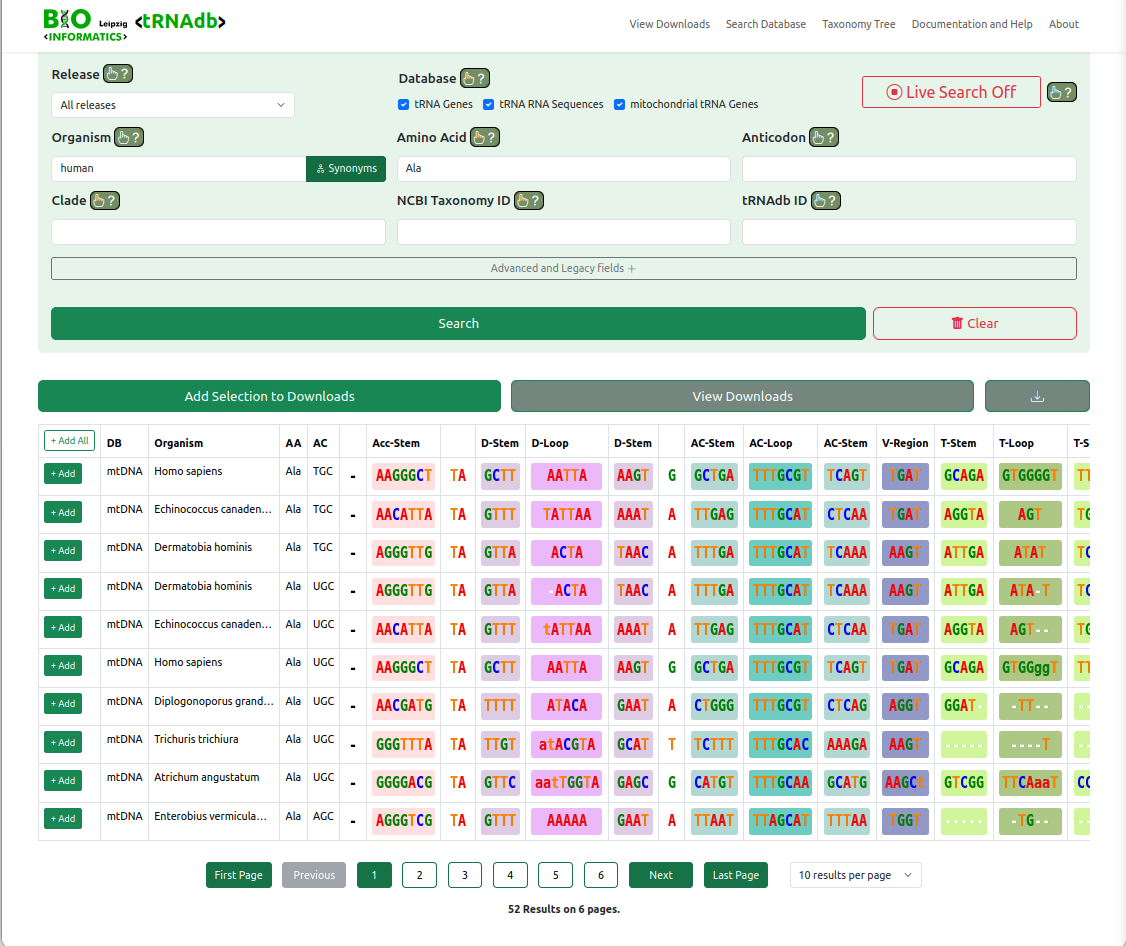
\includegraphics[width=0.4\textwidth]{Webserver_homo_ala.png}
  \caption{Example of the tRNAdb website, showing the first page of the
    results for a search for \emph{human} tRNAs for alanine, searching all
    three origins and using synonyms from NCBI
    taxonomy. \label{Fig:Website}}
\end{figure}
The main functionality of the website is the ``Search'' page which allows
users to filter tRNA by organism, origin (genomic DNA-based, mitochondrial
DNA-based, or RNA-based including modifications), amino acid, anticodon,
membership of taxonomic clades, external references (publications, genome
IDs, external datasources) as well as sequence motifs and structural
constraints. Species can be filtered precisely via NCBI taxonomy ID as well
as their scientific species name and species synonyms as annotated in the
NCBI taxonomy database. For every species with tRNA sequences present in
tRNAdb, their taxonomic lineage, as annotated in the NCBI taxonomy
database, is stored and tRNA belonging to a specific clade can be obtained
by using the ``Clade'' field of the search page.

Upon a successful search, the user is presented with a paginated list of
matching tRNA sequences with a snapshot of data available for every
sequence: origin, organism, amino acid, anticodon and its structurally
annotated nucleotide sequence (separated into acceptor stem, D-loop,
D-stem, etc.). Every result entry, or every entry matching the current
search request, can be stored in a temporary selection which can be
committed to persistent storage as a named collection for later access or
download.

A download manager allows exporting of individual collections, or every
saved collection, and offers customizable export options. Export of data in
\texttt{TSV}, \texttt{CSV}, \texttt{JSON}, and multi line FASTA format is
supported and every export can be further customized by selecting various
fields that are relevant to the individual user (e.g. sequence, structure,
annotated sequence, species name, taxonomic lineage, reference, and
more). FASTA export supports a customizable sequence identifier, for which
a preview is generated.
\begin{figure}
  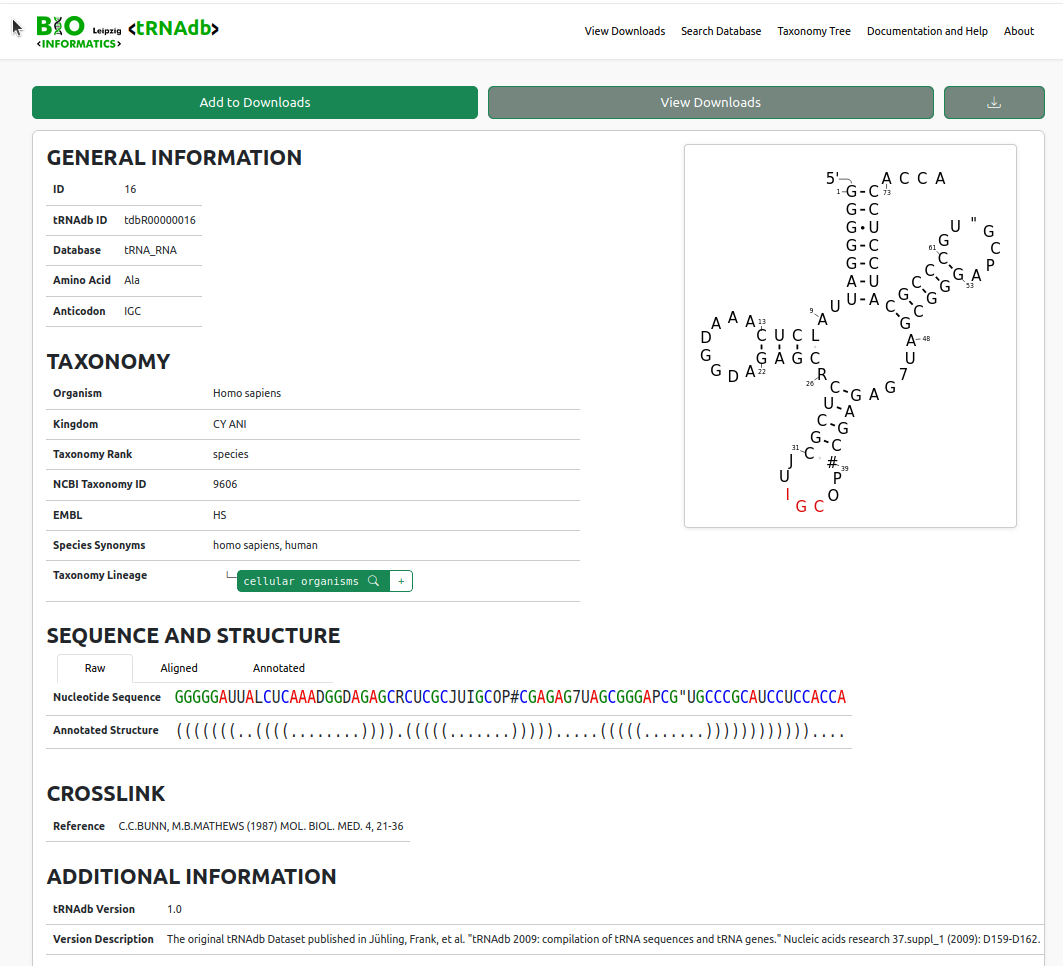
\includegraphics[width=0.45\textwidth]{Webserver_Detail_homo_ala.png}
  \caption{Example for the Details page of a \emph{homo sapiens} tRNA for alanine, including modifications\label{Fig:Detail}}
\end{figure}
For every tRNA sequence entry in our database, a "Details" page is
available (see Figure~\ref{Fig:Detail}). This page contains general
information (e.g., unique identifier, origin, amino acid, anticodon),
taxonomic information, sequence and structure, crosslinking information,
and additional metadata if available. Furthermore, a standardized
visualization of the secondary structure with a highlighted anticodon is
displayed for every entry.

We implemented a searchable taxonomy browser which displays an expandable
tree view of the NCBI taxonomic database. Every node in the taxonomy tree
is annotated with its scientific name according to the NCBI taxonomy as
well as its unique NCBI taxonomy ID. The taxonomy browser only displays
clades and species, for which there are tRNA sequences present in
tRNAdb. For every entry in the taxonomy browser, the number of tRNA
sequences separated by origin is displayed. Every node in the taxonomy
browser contains a link, which allows to search tRNAdb for sequences
belonging to this clade/species.

\section{Inclusion of new data}\label{sec3}

To include new data into tRNAdb, we used different approaches for different
types of tRNA for candidate identification, followed by alignment and
quality control for all candidate entries except for the modified
mitochondrial RNAs where the published assignment of bases to canonical
locations was used \cite{modtRNAbtaurus,humanmtRNA}, see
Figure\,\ref{workflow}.

\begin{figure}
  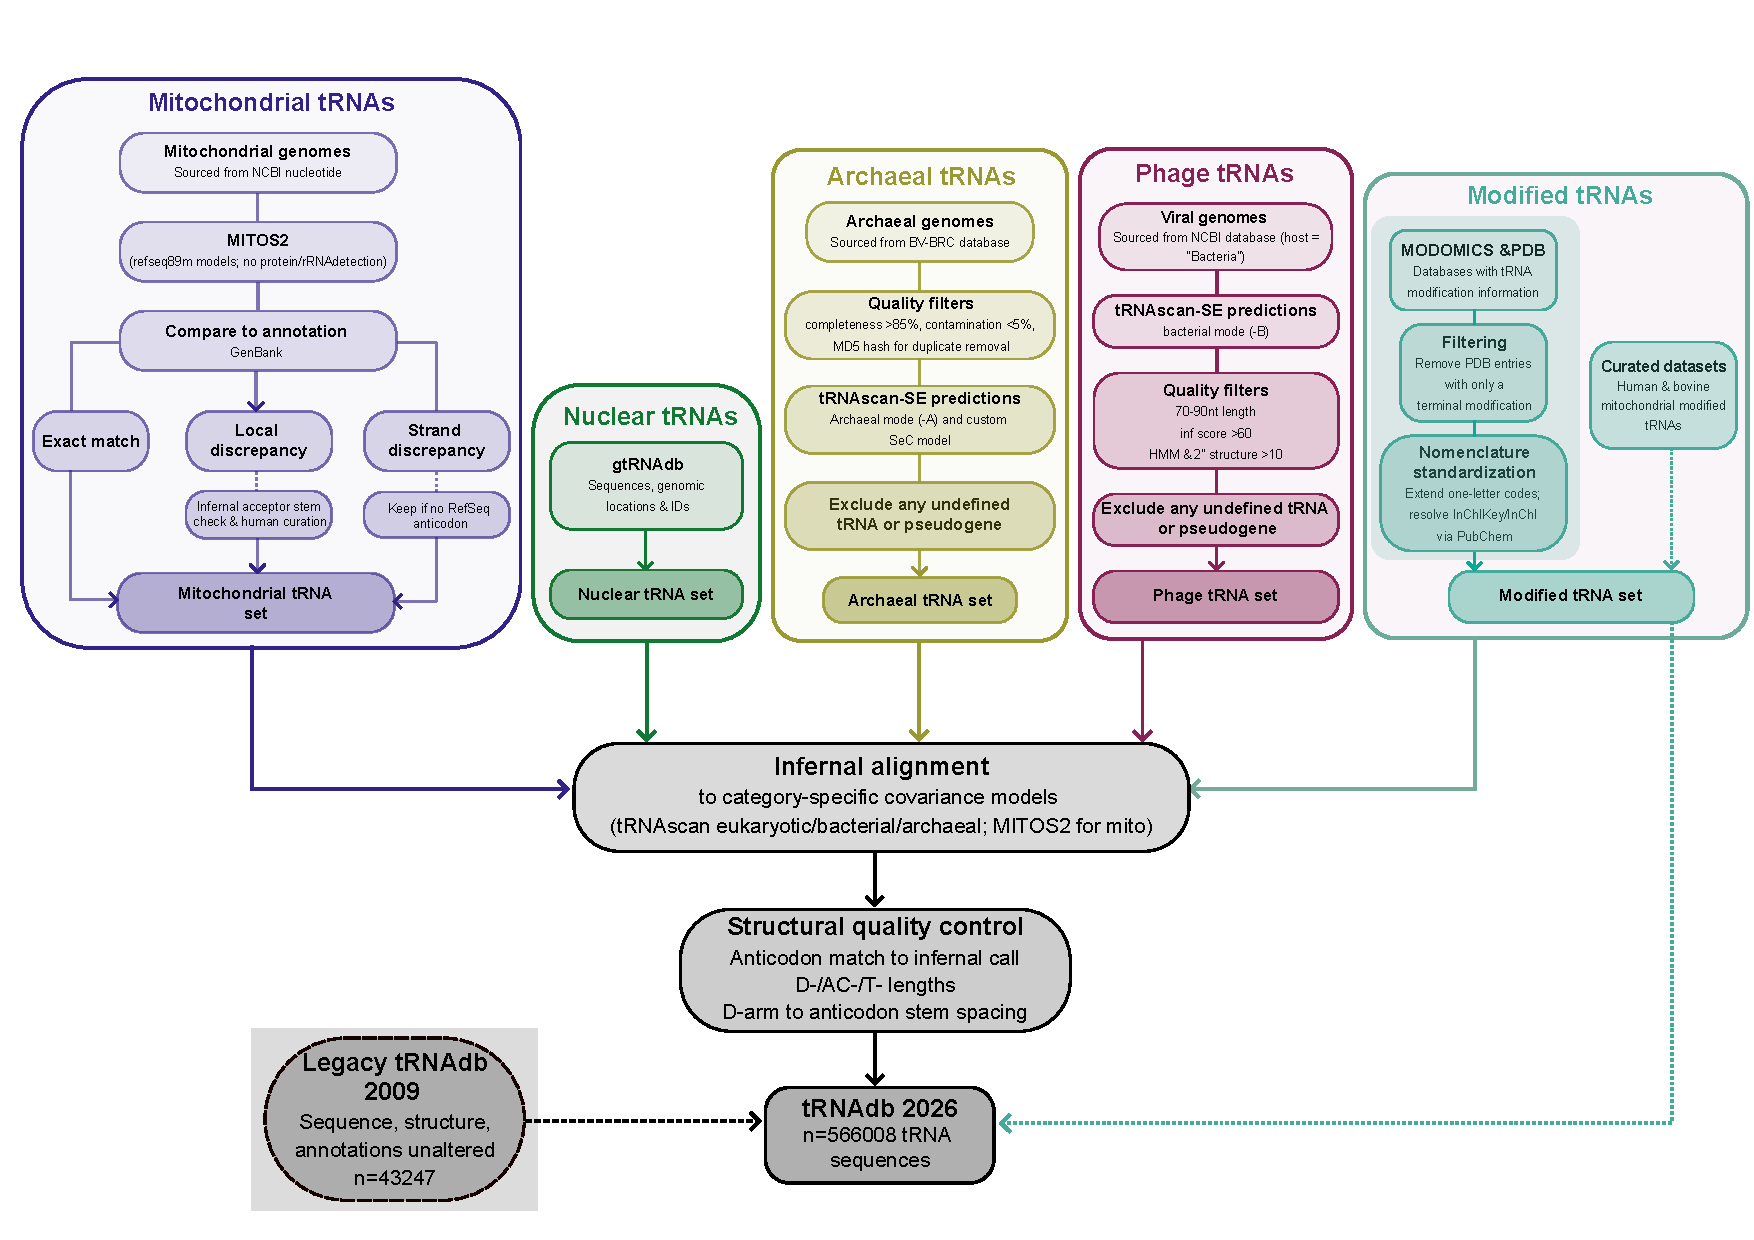
\includegraphics[width=0.47\textwidth]{workflow_figure.pdf}
  \caption{\label{workflow} Workflow for data inclusion. Different
    approaches for data acquisition and pre-filtering for different sources
    of tRNAs as well as common filtering and alignment steps are shown.}
\end{figure}

\subsection{Mitochondrial tRNAs}\label{subsecmitotRNA}

To expand the set of mitochondrial tRNAs included in the tRNAdb, a total of
$16\,630$ mitochondrial genome sequences, as well as their annotations were
obtained from NCBI Nucleotide~\cite{ncbinucleotide2024}, accessed October
2024. We used MITOS2~\cite{mitos2} without detection of proteins and rRNA
and the refseq89m models on each mitochondrial genome to search for
tRNAs. The predicted sequences were then compared to the NCBI
annotation. All tRNAs that matched exactly to the NCBI annotation were
added to tRNAdb. In case of discrepancies of location, we checked whether
the structure of the acceptor stem predicted by Infernal
1.1.4~\cite{infernal} passed human curation. In the affirmative case, the
sequence predicted by MITOS2 was deemed correct and included into the
database. In case of discrepancies in the assignment of the strand (reading
direction), we retained the MITOS2 prediction if no plausible anticodon
could be identified in the anticodon stem and loop of the NCBI annotation.
After filtering (see ``Alignment and quality control section'' below), this
resulted in 305\,905 novel predicted mtRNAs that were added to the
\texttt{tRNAdb}.

\subsection{Nuclear tRNAs}\label{subsecgenomictRNA}
Genomic tRNAs were sourced from the GtRNAdb, using the data release from
2024~\cite{gtrnadb}. Information retrieved included sequences, genomic
locations and genome IDs.  After filtering, $216\,856$ novel genomic tRNAs
were added to the tRNAdb.  GtRNAdb contains only a limited number of
archaeal tRNA entries (below 9\,000), covering a narrow taxonomic range
within archaea.  Since GtRNAdb also contains no virus-derived tRNAs, we
decided to further expand tRNAdb in these two areas.

\subsection{Archaeal tRNAs}

Archaeal genomes were sourced from the Bacterial and Viral Bioinformatics
Resource Center (BV-BRC) database~\cite{bvbrc2022}, accessed October
2024. Only high-quality genomes were retained for further analysis, and
genome quality was assessed by CheckM2 ($\geq$85\% complete, $<$5\%
contaminated)~\cite{checkm2}. These archaeal genomes cover a broad
taxonomic range and include all major archaeal superphyla (Asgard, DPANN,
TACK, and Euryarchaeota).  We did not rely on the BV-BRC annotation of tRNA
genes, as we found it inconsistent with predictions using the most
up-to-date version of tRNAscan-SE 2.0.12~\cite{tRNAscan}. Notably,
tRNA-Ile2 is often mislabelled as tRNA-Met in BV-BRC, the most frequent
mismatch we observed in isotype assignment (34\%). This likely reflects the
agmatidine wobble-base modification unique to archaea~\cite{tRNAscan},
highlighting the necessity to use domain-specific models.  Therefore, all
genomes were annotated using tRNAscan-SE in archaeal mode. Selenocysteine
tRNAs were identified using the SeC-specific covariance model, since it has
an atypical secondary structure~\cite{tRNAscan}. As independent validation,
all tRNAscan predictions were re-scored with Infernal~\cite{infernal}
against tRNAinf-arch and tRNAinf-arch-SeC models. After filtering (see
``Alignment and quality control section'' below), $21\,127$ tRNA genes from
228 unique archaeal genomes were added, of which 214 were not represented
in the 2009 tRNAdb, substantially expanding archaeal coverage relative to
the legacy dataset.

\subsection{Phage tRNAs}
Genome sequences of all viruses annotated with the host term ``Bacteria''
were obtained from NCBI Virus~\cite{ncbivirus}, accessed 17 August
2026. Putative tRNA genes were identified using tRNAscan-SE v2.0.12
\cite{tRNAscan} in bacterial mode.  Predicted tRNAs were retained only if
they were 70–90nt in length, had an overall tRNAscan-SE Bit Score $>$60,
and had both HMM and secondary-structure scores $>$10. Predictions with
undefined isotypes or classified as pseudogenes were excluded. After
filtering (see ``Alignment and quality control section'' below), $7\,099$
viral tRNA genes from $1\,558$ unique genomes were added to tRNAdb.

\subsection{tRNAs sequences including modifications}\label{subsecmodifiedtRNA}
Modified tRNA sequences, as well as their genomic variants, were obtained
from the MODOMICS \cite{modomics} database and the Protein Data Bank
(PDB)~\cite{pdb2000}.  Sequences retrieved from the PDB having only a
single modification located at the first or last base were not included
into the database.  In order to display alignments properly, legacy
one-letter codes for modifications were retained.  The dictionary of
one-letter codes for modifications was extended to include any that were
not present in the legacy tRNAdb 2009.  For these novel modifications, we
also identified the compound name using the PDB entry. The InChiKeys and
InChis were extracted from PubChem~\cite{pubchem2025} to check whether the
compound was already present in the MODOMICS database. A list of all
modifications with the one-letter codes used in tRNAdb and MODOMICS can be
found in the supplement and on the database webpage.  Mature mitochondrial
tRNA sequences from \emph{H.\ sapiens}~\cite{humanmtRNA} and \emph{B.\
  taurus}~\cite{modtRNAbtaurus} were added from the supplement of the
respective publications. The included canonical base numberings were used
directly for alignment and structural annotation.

\subsection{Alignment and quality control}
For all novel sequences, we used Infernal~\cite{infernal} to align them to
the respective tRNA covariance models (eukaryotic, bacterial or archaeal
models from tRNAscan for nuclear tRNAs, the respective MITOS2 models for
mitochondrial tRNAs). When an anticodon was annotated, we compared it to
the one identified by Infernal (at the center of the anticodon loop). To
filter tRNAs with suspicious structural features, we also checked the
length of the D-loops, AC-loops, and T-loops, as well as the number of
unpaired bases between D-stem and AC-stem. For the AC-loop, we used a
strict length of 7 nt. For the other structural features, we used the
maximum length of the respective structural feature in tRNAdb 2009, allowed
a single nucleotide difference in length (resulting in 18 and 28 nt for D
and T-loops respectively and 5 nt between D and AC-stem) and discarded a
total of 404 tRNAs that did not make one of the four thresholds. As a last
filtering step, all entries that were duplicates with respect to sequence
and taxonomic ID were unified when necessary, so that every
sequence/species pair in the tRNAdb is unique.

\section{Statistics}

The database lists $330\,261$ mitochondrial tRNA entries comprising
$219\,388$ unique sequences. The vast majority of these originate in
metazoa (see Fig.~\ref{Tax}a), which reflects the distribution of
mitochondrial genomes at the NCBI. The genomic part of the database
contains a total of $228\,955$ entries comprising $93\,257$ unique
sequences. The majority, precisely $149\,749$ entries, are bacterial
tRNAs. However, the difference of genomic tRNA representation in tRNAdb is
much smaller for unique sequences, see Fig.~\ref{Tax}b.

\begin{figure}
  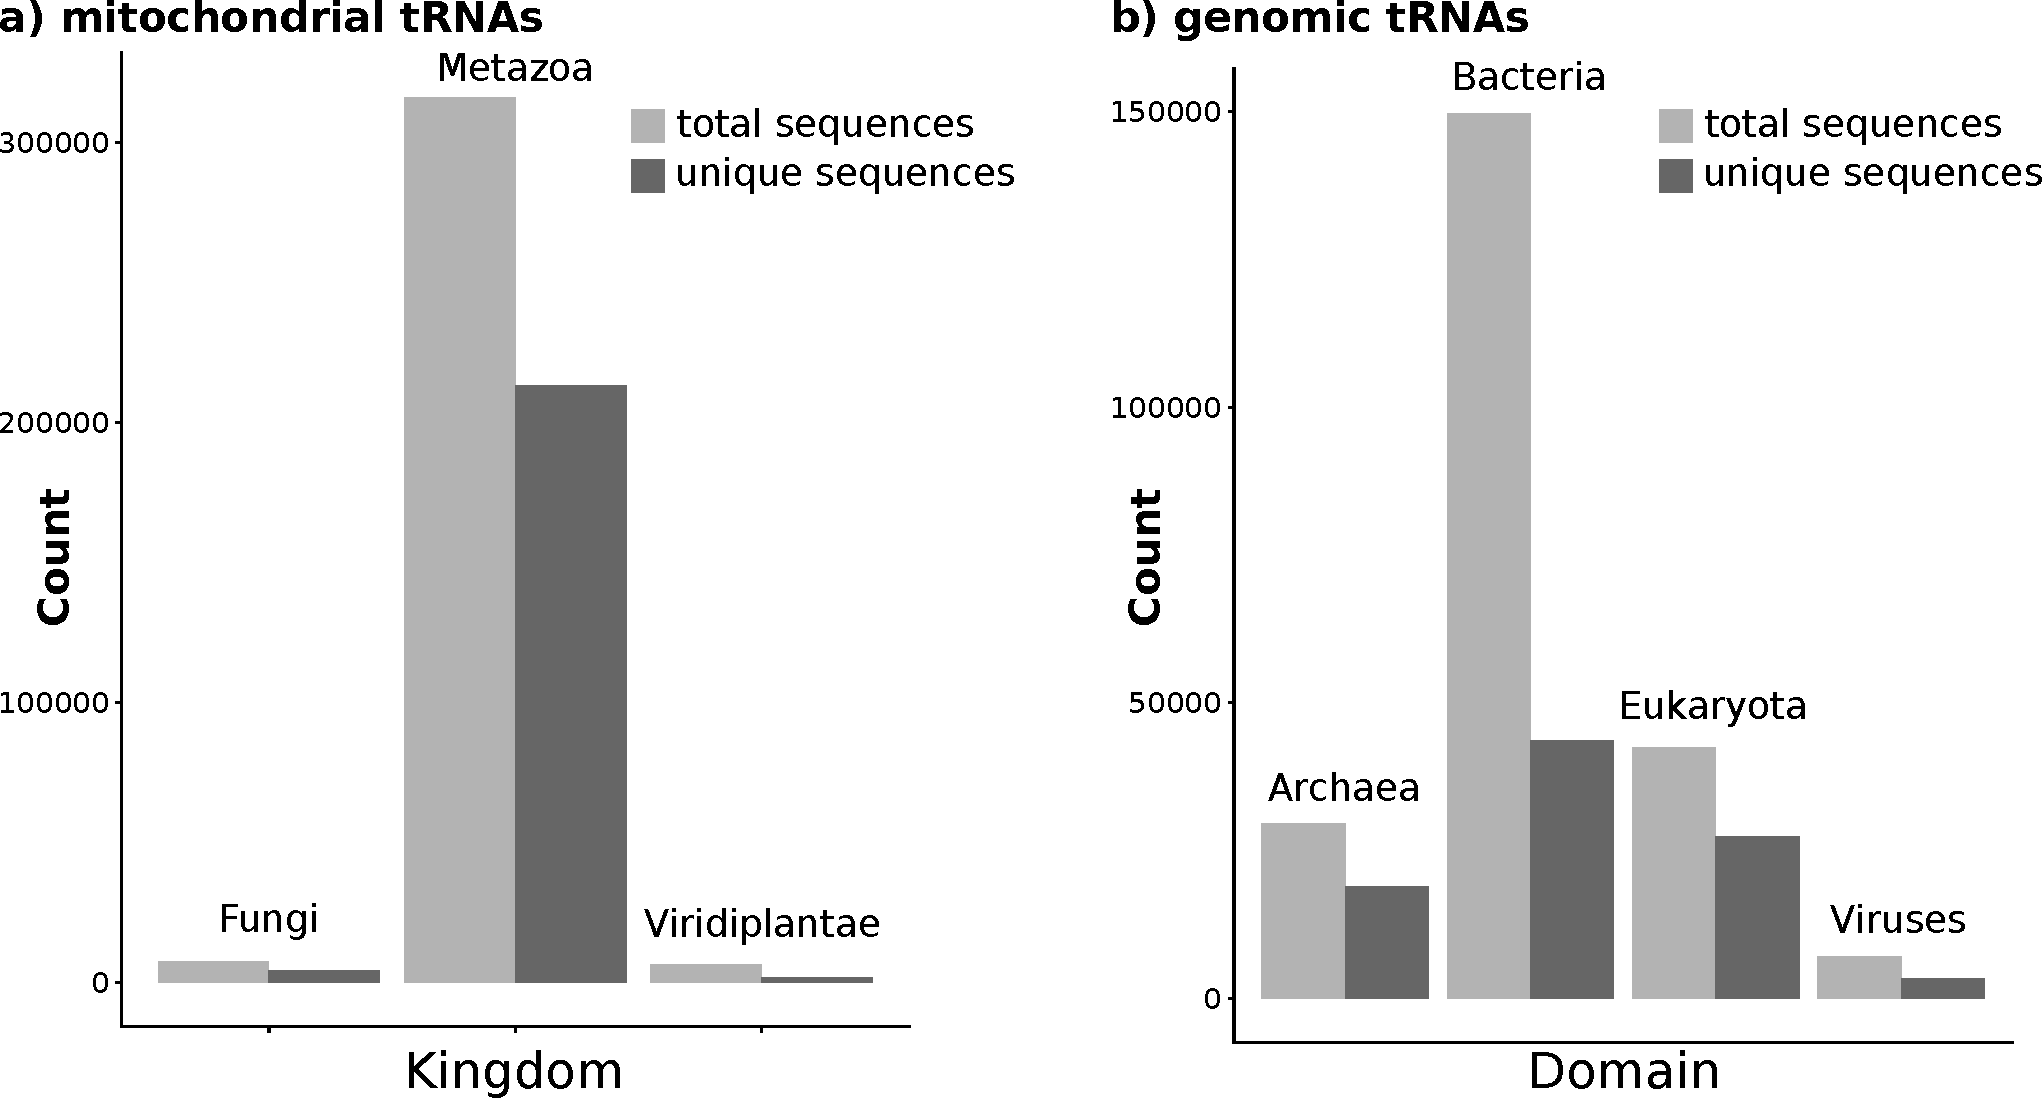
\includegraphics[width=0.45\textwidth]{taxonomicdistributions.pdf}
  \caption{\label{Tax}Number of tRNA sequences per clade. a: mitochondrial
    tRNAs at kingdom level. b: genomic tRNAs at domain level. Light gray
    shows number of all sequences, dark gray number of unique sequences.}
\end{figure}

Mitochondrial tRNAs show a relatively even distribution with respect to
their abundance, ranging from $14\,692$ entries for Glu to $16\,734$
entries for Met. The relatively even distribution can also be seen in the
unique sequences: Asp has the most with 12\,446, while Ser2 has the least
amount of unique sequences with 10\,184. The exception to these even
distributions are Leu1 (10\,857 entries, 6\,209 unique sequences) and to a
smaller extent Ser1 (12\,979 and 9\,457, resp.), which code for the two
amino acids that have two tRNAs in many mitochondria. Mitochondrial
tRNA-Lys is the only tRNA with a notable amount of two different anticodons
(Fig.~\ref{Aminoacidamounts}a).

In contrast, genomic tRNAs show a much wider variety in their
abundance. Leu, being the most abundant, has $23\,995$ entries and
$10\,233$ unique sequences. Besides the non-standard Suppressor and SeC
tRNAs, His has the fewest entries with $5\,290$ ($2\,305$ unique
sequences), while Phe and Trp have the fewest unique sequences with
$2\,093$ (in $5\,855$ and $5\,579$ entries, respectively). Notably, many
genomic tRNAs (Asn, Asp, Cys, His, Phe, Trp, Tyr) show a clear preference
for one codon (see Fig.~\ref{Aminoacidamounts}b). Not surprisingly, the
number of entries as well as the number of unique sequences per amino acid
strongly correlates with the number of frequent (n$> 100$) anticodons in
use for an amino acid ($\rho > 0.93, p< 10^{-8}$ for both).

\begin{figure}
  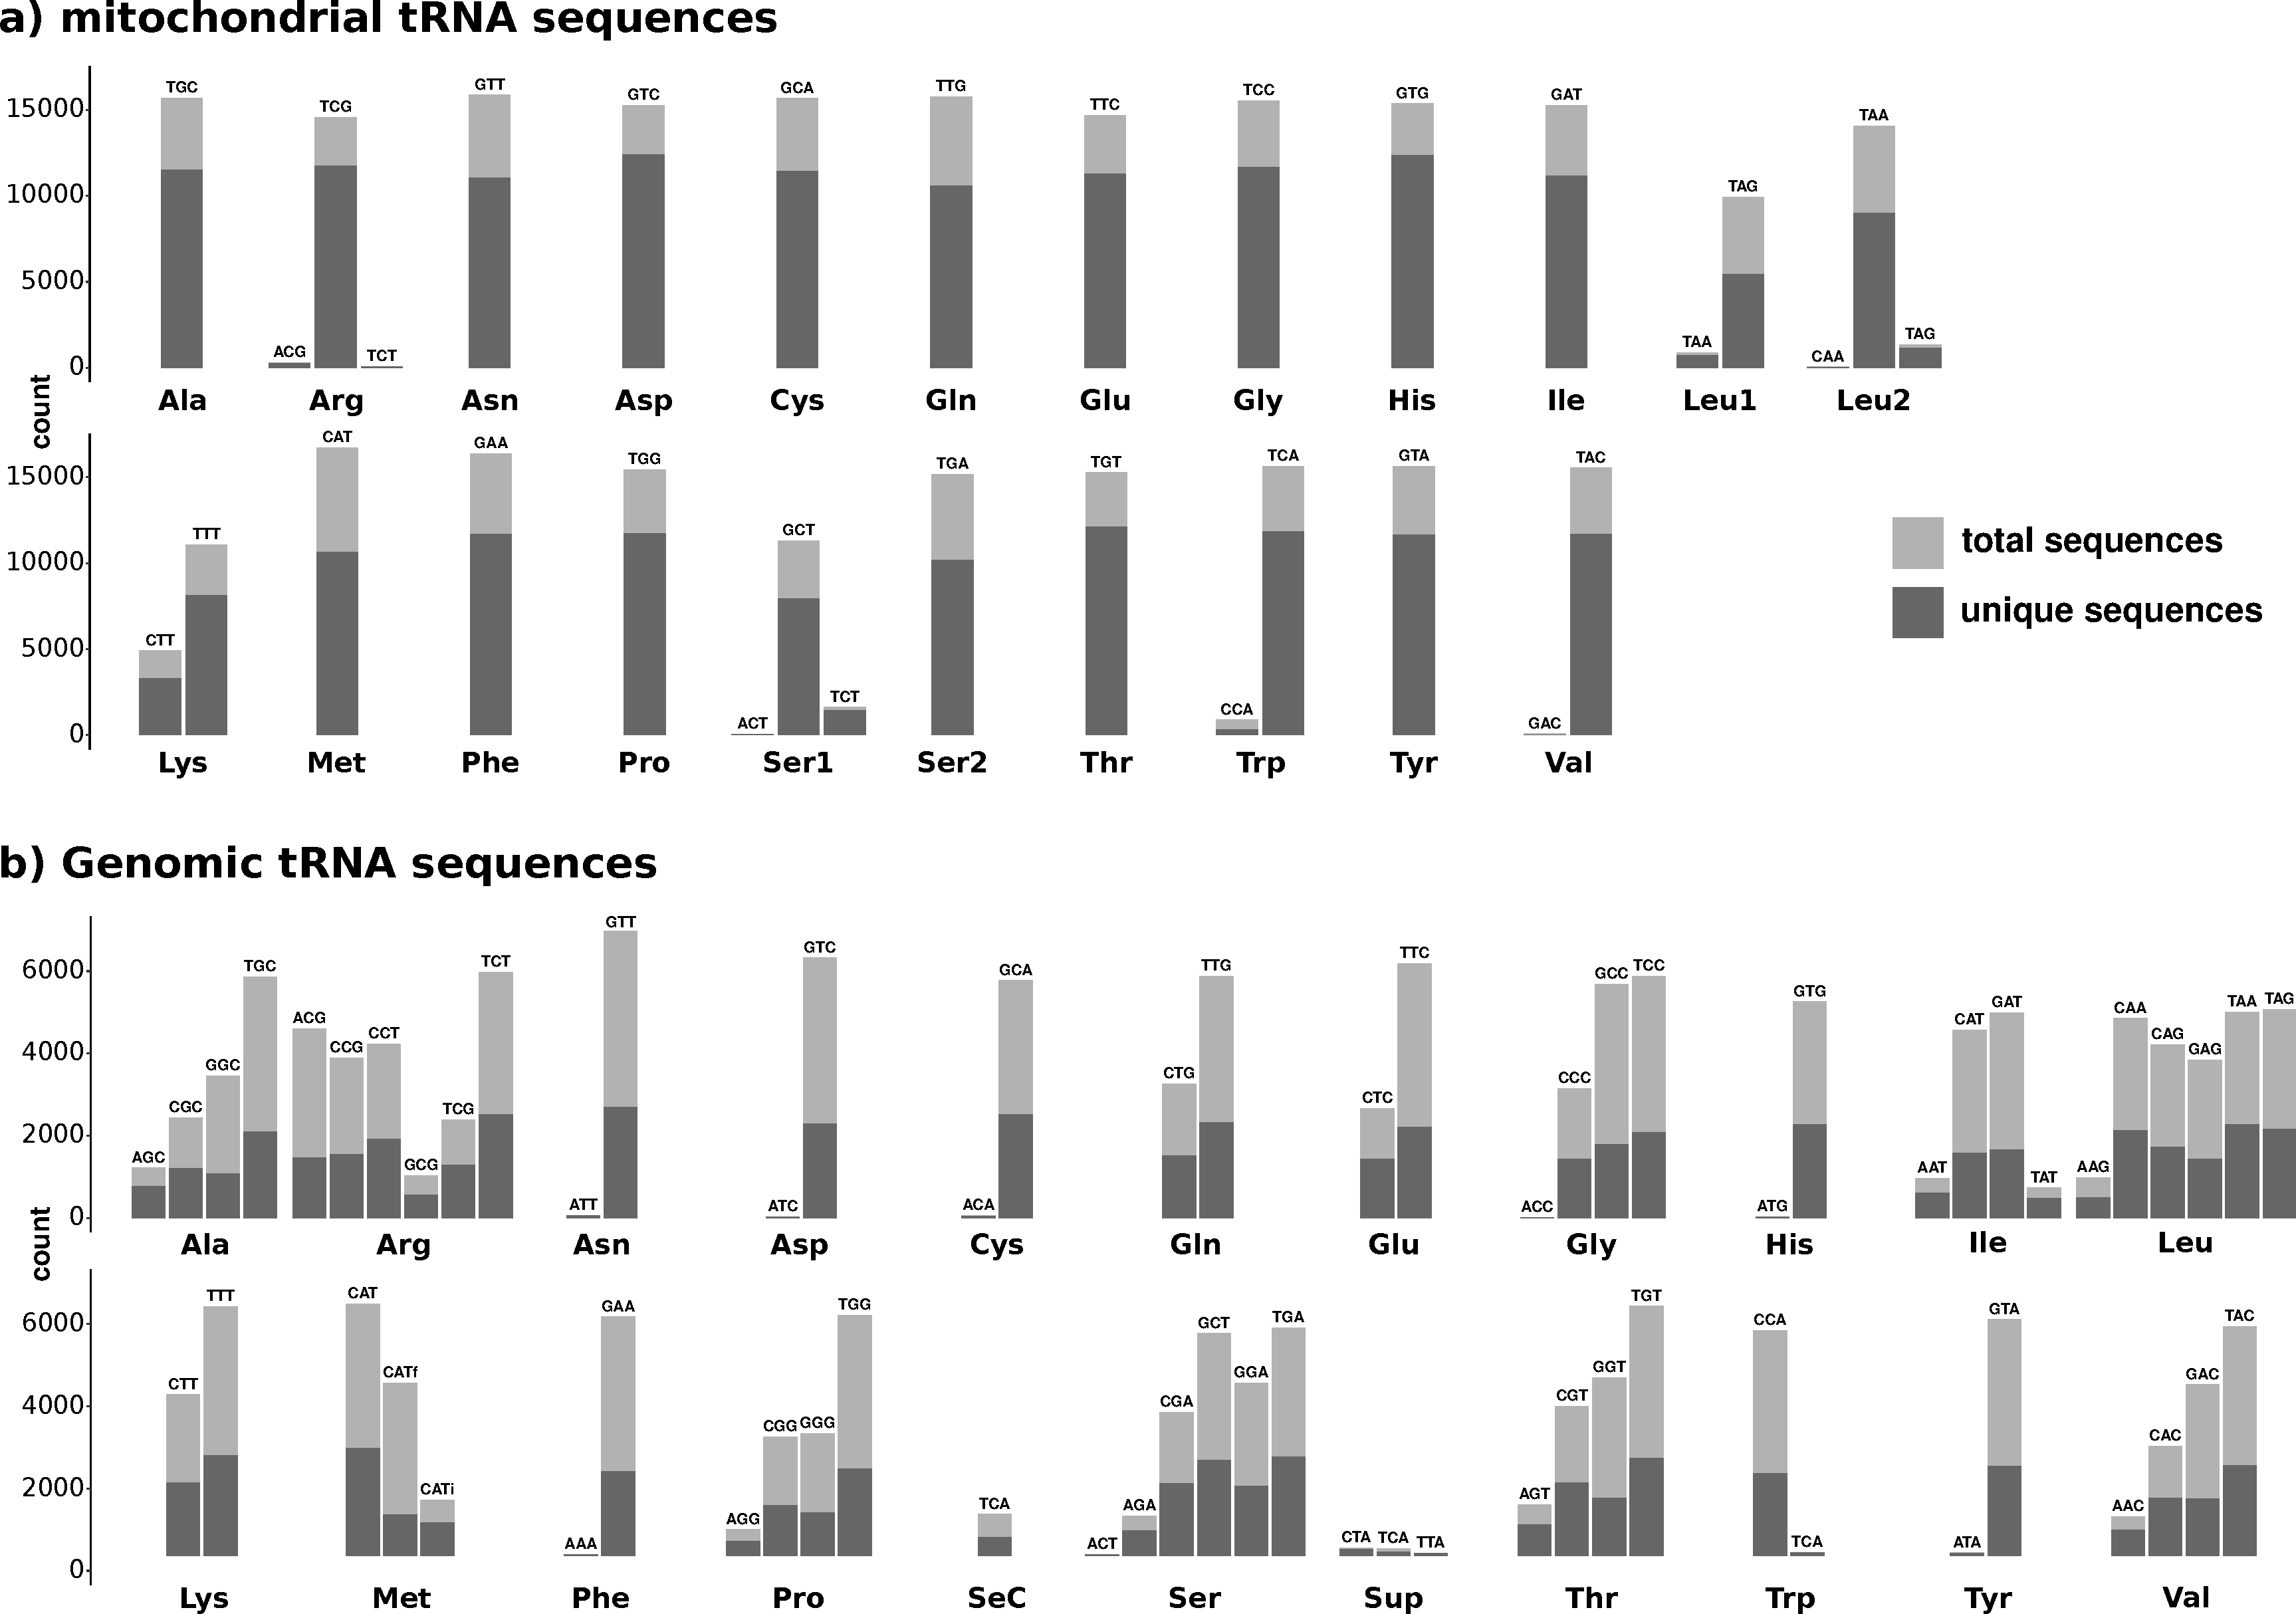
\includegraphics[width=0.4\textwidth]{MitoandGenomicAminoacidamounts.pdf}
  \caption{\label{Aminoacidamounts}Distribution of tRNAs per amino acid and
    anticodon. a) mitochondrial tRNA sequences b) genomic tRNA
    sequences. Light gray shows number of all sequences, dark gray number
    of unique sequences.}
\end{figure}

In comparison to the first version of tRNAdb, we greatly expanded sequences
belonging to clades that were either not included before, such as
mitchondrial tRNAs from viridiplantae or fungi, or had only very sparse
entries, such as archaea and viroidal genomic tRNAs (see
Fig.~\ref{species}). In total, tRNAdb\,2026 contains genomic entries from
$6\,086$ species, and mitochondrial entries from $15\,796$ different
species.
 \begin{figure}
  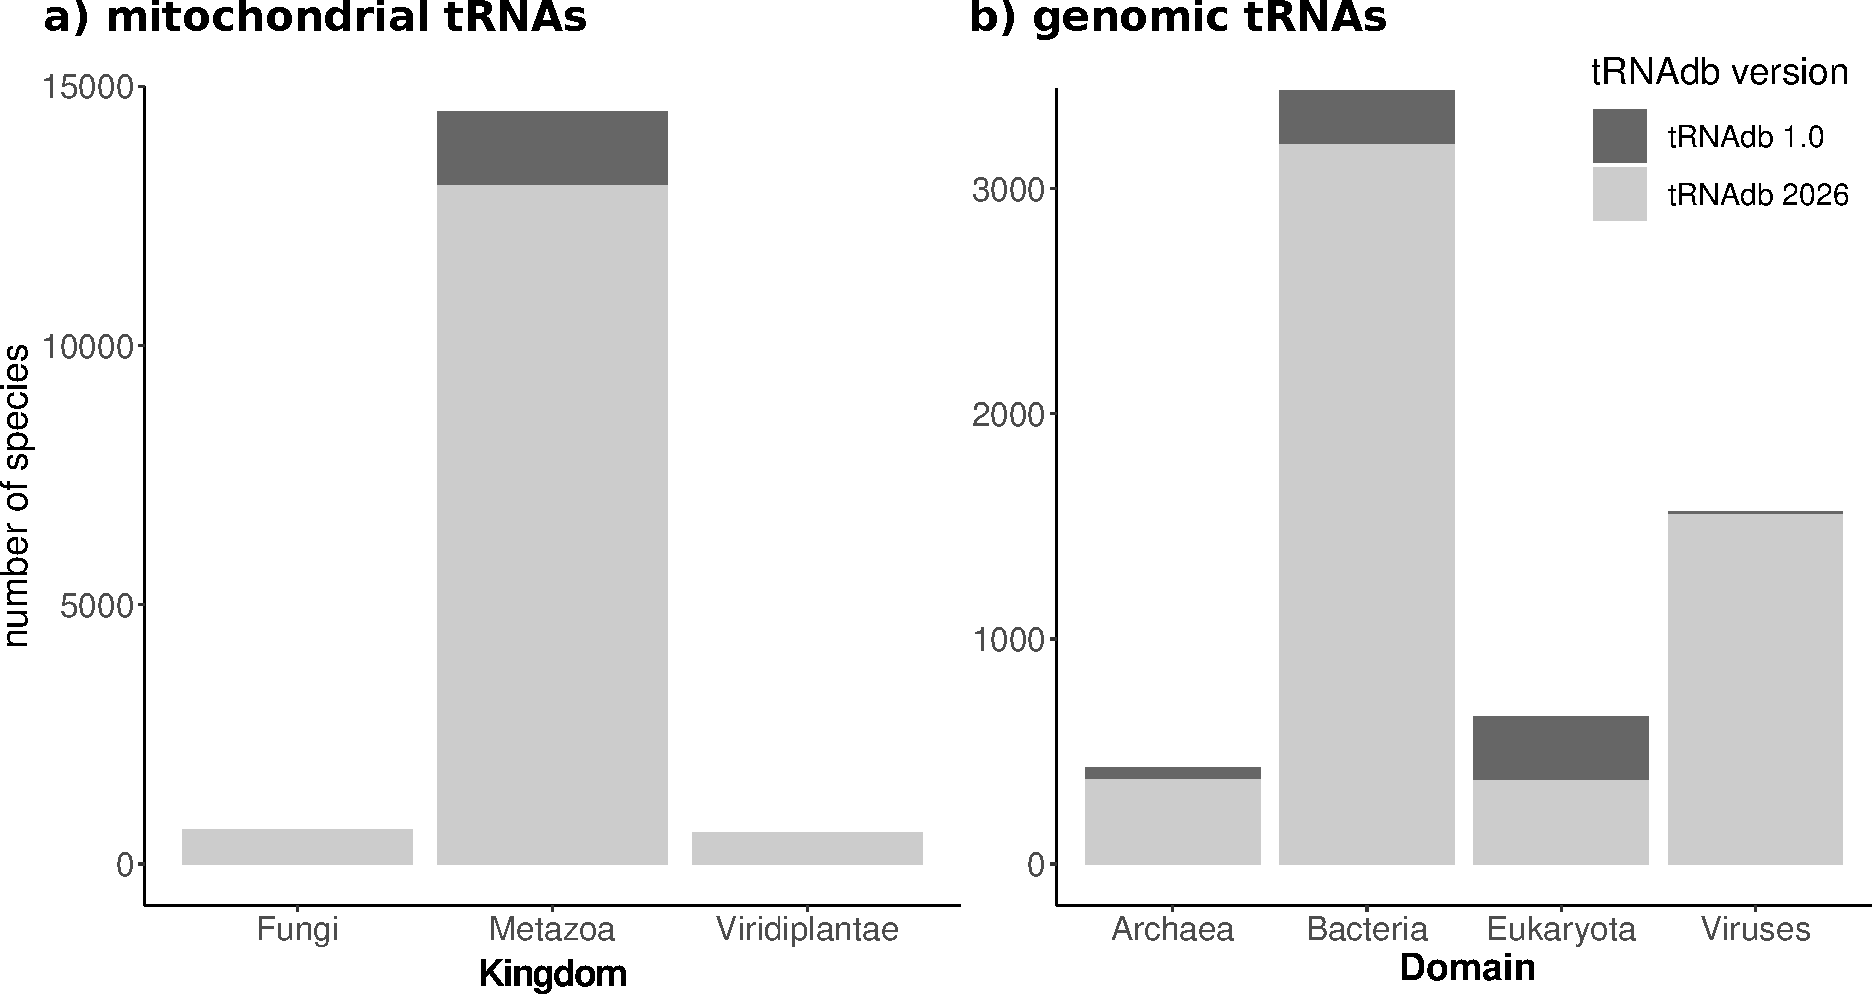
\includegraphics[width=0.4\textwidth]{Speciesdistribution.pdf}
  \caption{\label{species}Distribution of species included in the tRNAdb,
    seperated by clade. a) mitochondrial b) genomic tRNAs. Light gray shows
    number species in tRNAdb\,2026 only, dark gray number of species in
    tRNAdb 2009.}
\end{figure}

\section{Conclusion}

The updated tRNAdb has been expanded 11-fold and its infrastructure was
modernized throughout.  Alongside a redesigned web interface, it now
provides a public API and a considerable increase in the number of included
entries. Among these new entries now are modified mitochondrial tRNAs and,
for the first time, mitochondrial tRNAs from plants and fungi. tRNAdb thus
continues to serve as an important resource for the tRNA community.

However, because most entries in the tRNAdb stem from semi-automatic
annotation, fringe cases that deviate from established tRNA properties are
likely to be rejected, even though these are often of high biological
interest. We therefore rely on the community to report such sequences, so
they can be incorporated into future releases. This feedback may in turn
motivate updated search algorithms capable of capturing a broader range of
non-standard tRNAs.  To address such cases, we provide a web interface
where experts can submit entries of non-standard tRNAs that we will curate
and include into the database.

\section{Conflicts of interest}
C.L.B. is a co-founder and scientific advisor to Locus Biosciences and a
scientific advisor to Quidditas Therapeutics. The other authors declare
that they have no competing interests.

\section{Funding}
This work was funded in part by the Deutsche Forschungsgemeinschaft (DFG,
German Research Foundation) under Germany's Excellence Strategy -
EXC-3105/1 - 533765739, the Austrian Science Fund (FWF) F80 RNAdeco, the
German Federal Ministry of Research, Technology and Space (BMFTR) through
Leipzig RNA Bioinformatics Center (RBC) of the German Network for
Bioinformatics Infrastructure (de.NBI) sustained via Forschungszent\-rum
J\"{u}hlich.

\section{Data availability}
The data underlying the tRNAdb\,2026 are available in public repositories
like GtRNAdb, NCBI nucleotide and BV-BRC. Links to the sources as well as
all other relevant information are provided at the detail pages of the
webpage \url{https://tdb.bioinf.uni-leipzig.de/}.

\section{Author contributions statement}
\textbf{B.J.S.:} Software, Data curation, Writing – original draft, Writing
– review \& editing. \textbf{S.H.B.:} Conceptualization, Methodology,
Investigation, Data curation, Software, Writing – original draft, Writing –
review \& editing. \textbf{P.F.S.:} Conceptualization, Methodology, Writing
– original draft, Writing – review \& editing, Funding
acquisition. \textbf{E.C.:} Investigation, Writing – original draft,
Writing – review \& editing. \textbf{D.I.F} Validation, Writing – review \&
editing. \textbf{M.F.:} Investigation, Writing – review \&
editing. \textbf{T.S.:} Investigation, Data curation, Writing – review \&
editing. \textbf{F.J.:} Resources, Data curation, Writing – review \&
editing. \textbf{M.M.:} Resources, Data curation, Writing – review \&
editing. \textbf{J.P.:} Resources, Data curation, Writing – review \&
editing. \textbf{C.L.B.:} Supervision, Writing – review \& editing.


\bibliographystyle{oup-plain}
\bibliography{reference}

\end{document}

